\documentclass[journal]{IEEEtran}

\usepackage{amsmath,amssymb,amsfonts}
\usepackage{algorithmic}
\usepackage{graphicx}
\usepackage{textcomp}
\usepackage{xcolor}
\usepackage{booktabs}
\usepackage{cite}
\usepackage{url}
\usepackage{microtype}

\graphicspath{{figures/}}

\begin{document}

\title{Hybrid Visual Defect Inspection and Nominal-Only Adaptation: An Empirical Study of Detection Trade-Offs and Operational Constraints}

\author{Surya~Charan%
\thanks{Surya Charan is an independent computer vision researcher (email: suryacharan945@gmail.com).}%
}

\markboth{IEEE Transactions on Instrumentation and Measurement,~Vol.~XX, No.~X,~November~2026}%
{Charan: Hybrid Visual Defect Inspection and Nominal-Only Adaptation}

\maketitle

\begin{abstract}
Automated visual inspection in high-throughput manufacturing confronts an asymmetric operational penalty: undetected defect escapes can result in catastrophic downstream product failures, while excessive false alarms incur substantial scrap costs and line stoppages. Supervised deep convolutional classifiers achieve high precision on recurring, anticipated defect classes but frequently fail on rare, novel defect morphologies. Conversely, unsupervised patch-based anomaly detectors capture arbitrary distribution shifts without defect supervision, but can suffer from elevated false-positive rates due to natural intra-class surface variance. 

In this paper, we conduct an empirical investigation into a dual-branch hybrid inspection architecture combining a supervised visual classifier (EfficientNet-B0 v3) with an unsupervised patch-distribution memory bank (PatchCore), characterizing the concrete trade-offs, computational overhead, and adaptation boundaries inherent to practical deployment. On an audited development-exposed benchmark of 856 industrial specimens from the MVTec Anomaly Detection dataset, the hybrid decision policy (logical OR) increased defect recall from 82.24\% to 90.88\%, successfully capturing 54 defect instances missed by the standalone supervised model (slashing escapes from 111 to 57), while increasing false alarms from 1 to 12 (false positive rate rising from 0.43\% to 5.19\%). 

To assess cross-domain transfer without defect supervision, we independently evaluated the patch-level memory pipeline on the untouched Visual Anomaly (VisA) Cashew benchmark using 350 domain-specific nominal specimens for registration and 50 held-out nominals for threshold calibration ($\tau_{\text{p99}} = 1.7452$). Across 200 independent test specimens (100 nominal, 100 defective), the adapted model achieved an image-level AUROC of 0.9237 [95\% CI: 0.8852, 0.9565], an image-level AUPRC of 0.9270, and a full-census pixel-level AUROC of 0.9930 across 10.03 million evaluated pixels. Operating at the locked 99.5th-percentile calibration threshold enforced a high specificity of 98.00\% (2.00\% false alarm rate); however, granular sensitivity profiling revealed a 43.00\% defect escape rate concentrated heavily in fine surface flaws: gross structural breaks and boundary distortions achieved 100\% recall (6/6), dark voids achieved 85.0\% recall (17/20), whereas hairline scratches and same-color depressions yielded escape rates of 93.3\% (1/15 recall) and 100.0\% (0/10 recall), respectively. 

Execution profiling on consumer multi-core CPU hardware confirmed memory registration in 392.25~s (27,440 coreset tokens, 40.2~MB index) and deterministic forward inference of 392.5~ms median (p95: 438.1~ms), confirming computational feasibility for discrete inspection stations with cycle times $\ge 1.5$~s. Our findings demonstrate that while nominal-only adaptation provides robust baseline containment and high localization precision, automated unassisted sorting requires multi-scale optical resolution or secondary verification to mitigate the severe tension between false-alarm suppression and hairline flaw escapes.
\end{abstract}

\begin{IEEEkeywords}
Industrial defect inspection, anomaly detection, PatchCore, EfficientNet, decision fusion, quality control, operational trade-offs, VisA benchmark.
\end{IEEEkeywords}

\IEEEpeerreviewmaketitle

\section{Introduction}
\IEEEPARstart{A}{utomated} surface defect inspection represents a critical quality assurance pillar across precision manufacturing, including semiconductor fabrication, automotive stamping, pharmaceutical packaging, and consumer goods sorting~\cite{weimer2016design,kumar2008computer}. In modern production environments, visual quality gating operates under an asymmetric cost matrix. A Type~II error (false negative / defect escape) delivers substandard or structurally compromised components to downstream assembly lines or end customers, risking catastrophic equipment damage, safety hazards, and costly product recalls. Conversely, a Type~I error (false positive / false alarm) falsely flags conforming product as defective, inducing unnecessary component scrap, excessive manual reinspection labor, and disruptive production line stoppages~\cite{kumar2008computer,duda2001pattern}.

In recent years, deep learning methodologies for automated visual inspection have bifurcated into two primary paradigms:
\begin{enumerate}
    \item \textbf{Supervised Visual Classification:} Deep convolutional neural networks (CNNs) and Vision Transformers trained on extensive annotated libraries of defective and conforming components~\cite{tan2019efficientnet,weimer2016design}. When evaluated against recurring, pre-defined flaw topologies, supervised models deliver exceptional precision and near-zero false-alarm rates. However, they rely on a closed-world assumption: when presented with novel, unmodeled defect geometries, anomalous foreign materials, or unrepresented physical damage, supervised classifiers exhibit overconfident misclassifications, leading to severe defect escapes~\cite{weimer2016design}.
    \item \textbf{Unsupervised Anomaly Detection:} Systems trained exclusively on nominal (defect-free) component imagery to model the distribution of normal appearances, such as memory-bank nearest-neighbor methods~\cite{roth2022towards,defard2021padim,cohen2020sub}. Because they require no defect annotations, these methods theoretically detect arbitrary deviations from nominality. However, in factory environments characterized by natural intra-class texture variations, slight illumination drifts, and part positioning jitter, purely unsupervised models frequently suffer from elevated false-alarm rates that factory operators cannot tolerate~\cite{roth2022towards,weimer2016design}.
\end{enumerate}

To harness the complementary strengths of both paradigms, industrial practitioners frequently explore dual-branch hybrid architectures, combining a supervised classifier with an unsupervised anomaly detector via logical disjunction (OR-logic)~\cite{weimer2016design}. Under this regime, a specimen is quarantined if either branch flags a potential flaw. While the conceptual appeal of such hybrid gating is widely recognized, literature in applied instrumentation and measurement rarely quantifies the precise operational penalty curve: how many false alarms must a factory absorb to reduce defect escapes by a given margin? Furthermore, while unsupervised methods claim rapid adaptation to new manufacturing lines, empirical studies evaluating nominal-only adaptation on completely unseen, out-of-distribution industrial substrates under strict audit protocols remain scarce.

\subsection{Contributions of This Work}
In this paper, we present an empirical evaluation of hybrid defect detection and nominal-only category adaptation under concrete operational and hardware constraints. Rather than asserting architectural or mathematical novelty, the primary scientific and engineering contributions of this work are:
\begin{enumerate}
    \item \textbf{Direct Empirical Quantification of the Hybrid Operating Trade-Off:} On an audited development-exposed benchmark of 856 industrial images (MVTec AD~\cite{bergmann2021mvtec}), we quantify the exact cost curve of dual-branch decision fusion: pairing an EfficientNet-B0 v3 classifier~\cite{tan2019efficientnet} with a PatchCore memory bank~\cite{roth2022towards} captured \textbf{54 defect instances missed by the supervised model alone} (reducing missed defects from 111 to 57; recall rising from 82.24\% to 90.88\%), at the operational expense of \textbf{11 additional false alarms} (increasing false alarm rate from 0.43\% to 5.19\%).
    \item \textbf{First-Party Independent Adaptation Validation:} We execute a strictly isolated, out-of-distribution evaluation of nominal-only PatchCore registration on the untouched Visual Anomaly (VisA) Cashew benchmark~\cite{zou2022spot}, using 350 nominal registration images and 50 held-out nominal calibration images. Across 200 independent test specimens (100 nominal, 100 defective), the system achieved an image-level AUROC of \textbf{0.9237} [95\% CI: 0.8852, 0.9565], an image-level AUPRC of \textbf{0.9270}, and a full-census pixel-level AUROC of \textbf{0.9930} across 10.03 million evaluated pixels.
    \item \textbf{Granular Defect-Type Sensitivity Profiling:} We unpack aggregate AUROC metrics across 16 fine-grained defect morphologies in the VisA Cashew benchmark, exposing the boundary conditions of patch-distance anomaly scoring. While macroscopic deformities and gross structural breaks achieved \textbf{100\% recall} (6/6), hairline surface scratches and subtle same-color indentations yielded catastrophic escape rates of \textbf{93.3\%} (1/15 recall) and \textbf{100.0\%} (0/10 recall) under factory-grade false-alarm constraints ($\tau_{\text{p99}}$).
    \item \textbf{Hardware Feasibility Profiling on Consumer CPU:} We demonstrate that memory-bank adaptation and deterministic inference are achievable on standard multi-core CPU workstations without GPU acceleration: registration of 350 nominal images completed in \textbf{392.25~s} (40.2~MB memory footprint), with deterministic per-image inference latencies of \textbf{392.5~ms median} (p95: 438.1~ms), confirming viability for discrete manufacturing stations with cycle times $\ge 1.5$~s.
    \item \textbf{Rigorous Accounting of Engineering Dead-Ends:} We transparently document negative results encountered during development, specifically the failure of Context-Preserving Normalization Dropout (CPND) to improve generalization and the severe optimization instability of Multi-Axis Cross-Branch Attention (MACBA), establishing verified guardrails for future applied research.
\end{enumerate}

\begin{figure*}[t]
\centering
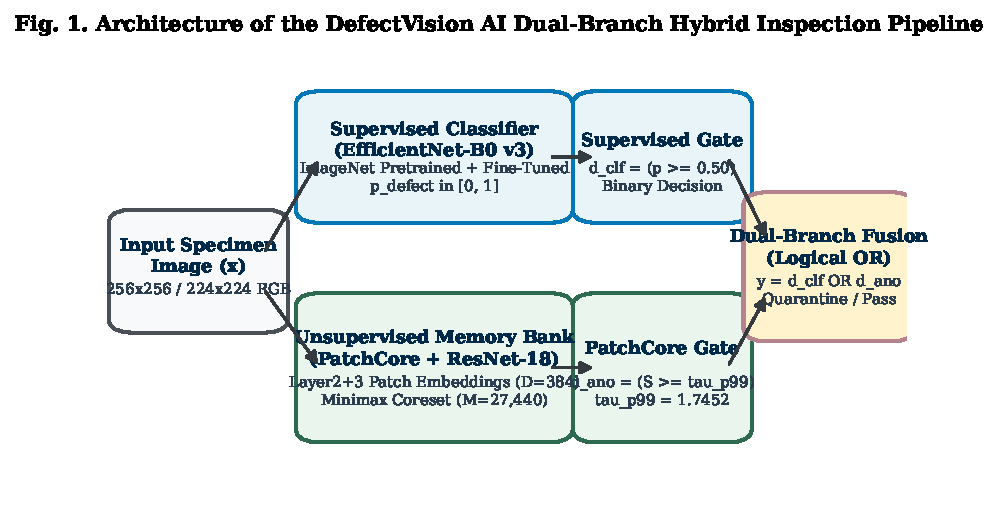
\includegraphics[width=0.88\textwidth]{fig1_architecture.pdf}
\caption{Architecture of the DefectVision AI dual-branch hybrid inspection pipeline combining supervised classification (EfficientNet-B0 v3) and unsupervised patch anomaly memory (PatchCore) via logical OR decision fusion.}
\label{fig:architecture}
\end{figure*}

\section{Related Work}

\subsection{Supervised Defect Classification}
Supervised deep convolutional neural networks have been widely applied to automated visual inspection across diverse manufacturing sectors~\cite{weimer2016design,kumar2008computer}. Architectures such as ResNet~\cite{he2016deep} and EfficientNet~\cite{tan2019efficientnet} optimize depth, width, and resolution scaling to maximize classification accuracy while maintaining parameter efficiency. EfficientNet-B0, parameterized with approximately 5.3 million weights, provides an exceptional balance of representational capacity and inference speed, making it widely adopted in industrial workstations~\cite{tan2019efficientnet}. However, supervised classifiers operate under the fundamental vulnerability of closed-world training~\cite{weimer2016design}: when presented with novel defect classes, foreign contaminants, or structural variations absent from the training split, their posterior probability estimates $p(\text{defective}|x)$ become unreliable, frequently producing overconfident false-negative predictions that allow critical defects to escape inspection~\cite{weimer2016design}.

\subsection{Unsupervised Anomaly Detection and Localization}
To eliminate dependence on rare and costly defect annotations, unsupervised visual anomaly detection models the manifold of nominal appearance using defect-free imagery exclusively~\cite{roth2022towards,bergmann2021mvtec}. Early approaches utilized deep autoencoders, variational autoencoders (VAEs), and generative adversarial networks (GANs) to compute pixel-level reconstruction error~\cite{bergmann2021mvtec}. However, generative reconstruction models frequently suffer from identity shortcutting, where anomalous features are blurrily reconstructed, degrading localization sharpness~\cite{roth2022towards}.

More recently, feature-embedding methods leveraging pre-trained deep representations have established state-of-the-art benchmarks in industrial anomaly detection~\cite{roth2022towards,defard2021padim,cohen2020sub}. SPADE~\cite{cohen2020sub} introduced multi-scale nearest-neighbor feature retrieval using deep pyramid correspondences. PaDiM~\cite{defard2021padim} fit multivariate Gaussian distributions to localized patch embeddings across nominal cohorts, enabling fast inference but constraining representation to unimodal distributions. PatchCore~\cite{roth2022towards} significantly advanced the state of the art by constructing an unconstrained memory bank of neighborhood-aware patch-level feature vectors extracted from intermediate stages of an ImageNet-pretrained convolutional backbone. By applying a greedy minimax facility location coreset reduction, PatchCore condenses the patch memory bank to a small fraction of representative tokens while preserving coverage of the nominal manifold, yielding superior image-level and pixel-level anomaly AUROC~\cite{roth2022towards}.

\subsection{Industrial Benchmarks: MVTec AD and VisA}
Empirical progress in visual anomaly detection has been driven by standardized real-world benchmarks. The MVTec Anomaly Detection (MVTec AD) dataset~\cite{bergmann2021mvtec} comprises 5,354 high-resolution images across 15 industrial manufacturing categories (10 rigid objects, 5 textures), providing a diverse testbed of real defect topologies. However, because MVTec AD has been extensively utilized for hyperparameter tuning and model optimization across hundreds of published papers since 2019, evaluations conducted on MVTec test splits must be carefully audited to distinguish development-exposed performance from genuine out-of-distribution adaptation~\cite{bergmann2021mvtec}. 

The Visual Anomaly (VisA) dataset, introduced by Zou et al.~\cite{zou2022spot}, provides 10,821 images across 12 categories, encompassing complex structures, multiple distinct objects per image, and natural organic goods (e.g., \texttt{cashew}). VisA represents a substantially more challenging benchmark for anomaly detection due to natural intra-class morphological variance, irregular object contours, and subtle low-contrast flaw topologies~\cite{zou2022spot}.

\section{System Methodology and Architecture}
The DefectVision AI architecture integrates two decoupled inspection engines executing concurrently on an incoming component image: a supervised defect classifier (EfficientNet-B0 v3) and an unsupervised patch-distribution memory bank (PatchCore). The overall pipeline is illustrated in Fig.~\ref{fig:architecture}.

\subsection{Unsupervised Patch-Level Memory Pipeline (PatchCore)}
The unsupervised branch implements the PatchCore paradigm~\cite{roth2022towards} utilizing a permanently frozen ResNet-18 backbone pre-trained on ImageNet-1K.

\subsubsection{Feature Extraction}
Given an input image $x \in \mathbb{R}^{3 \times H \times W}$ resized to $224 \times 224$, patch representations are extracted from intermediate residual stages: \texttt{layer2} (stride 8, 128 channels) and \texttt{layer3} (stride 16, 256 channels). To capture spatial context, each feature map is smoothed via $3 \times 3$ local adaptive average pooling with stride 1. The feature maps are bilinearly interpolated to a common spatial resolution ($28 \times 28$) and concatenated channel-wise, producing a dense grid of $N_p = 28 \times 28 = 784$ patch feature vectors:
\begin{equation}
m(i,j) \in \mathbb{R}^{D}, \quad D = 128 + 256 = 384
\end{equation}

\subsubsection{Greedy Minimax Coreset Subsampling}
For a nominal registration cohort of $K_{\text{reg}}$ images, the total extracted patch collection $\mathcal{M}_{\text{raw}} = \bigcup_{k=1}^{K_{\text{reg}}} \mathcal{M}_k$ contains $|\mathcal{M}_{\text{raw}}| = K_{\text{reg}} \times 784$ feature vectors. Storing and searching this unconstrained collection introduces excessive memory and latency overhead. We apply the iterative greedy $k$-Center minimax facility location algorithm~\cite{roth2022towards} to select a representative subset $\mathcal{M}_{\text{coreset}} \subset \mathcal{M}_{\text{raw}}$ of size $M$:
\begin{equation}
m^* = \arg\max_{m \in \mathcal{M}_{\text{raw}} \setminus \mathcal{M}_{\text{coreset}}} \min_{c \in \mathcal{M}_{\text{coreset}}} \|m - c\|_2
\end{equation}
Subsampling at a target coreset ratio $\kappa = 0.10$ condenses the memory bank by an order of magnitude while preserving coverage of the nominal patch manifold~\cite{roth2022towards}.

\subsubsection{Fast Nearest-Neighbor Indexing}
The coreset feature vectors are indexed using an exact Euclidean distance flat index (\texttt{IndexFlatL2}) via the FAISS library~\cite{johnson2019billion} executing natively on multi-threaded CPU hardware.

\subsubsection{Anomaly Scoring and Heatmap Generation}
At test time, patch vectors $p \in \mathcal{M}_{\text{test}}$ extracted from an input image are queried against $\mathcal{M}_{\text{coreset}}$. The patch-level anomaly score is defined as the Euclidean distance to its nearest nominal neighbor:
\begin{equation}
s(p) = \min_{c \in \mathcal{M}_{\text{coreset}}} \|p - c\|_2
\end{equation}
The patch anomaly scores are reshaped to a $28 \times 28$ spatial grid, bilinearly upsampled to $224 \times 224$, and convolved with a 2D Gaussian smoothing kernel ($\sigma = 4.0$) to generate the continuous anomaly heatmap $\mathcal{A}(u,v)$. The specimen-level anomaly score $S_{\text{img}}$ is defined as the maximum spatial anomaly score across the smoothed map:
\begin{equation}
S_{\text{img}} = \max_{(u,v)} \mathcal{A}(u,v)
\end{equation}

\subsection{Statistical Decision Threshold Calibration}
To establish an operational binary decision boundary without defect supervision, we enforce a strict quantile-based calibration protocol. A cohort of $K_{\text{cal}}$ nominal specimens held out from coreset registration is processed through the memory pipeline to compute nominal baseline scores. The operational decision threshold $\tau_{\text{p99}}$ is set to the empirical 99.5th percentile of the calibration score distribution:
\begin{equation}
\tau_{\text{p99}} = \text{Percentile}\left(\{S_{\text{cal},1}, S_{\text{cal},2}, \dots, S_{\text{cal},K_{\text{cal}}}\}, 99.5\right)
\end{equation}
This deterministic calibration locks the decision boundary to enforce a theoretical nominal false-alarm rate $\le 1.0\%$ prior to evaluating any unseen test data.

\subsection{Supervised Visual Classification Pipeline (EfficientNet-B0 v3)}
The supervised branch executes a fine-tuned EfficientNet-B0 classifier~\cite{tan2019efficientnet}. Input images are resized to $256 \times 256$, normalized using ImageNet channel statistics, and processed through mobile inverted bottleneck convolutions (MBConv) to produce a 1280-dimensional global representation vector. A fully connected classification head with softmax activation outputs the posterior defect probability $p_{\text{defect}} \in [0, 1]$. The binary supervised decision is parameterized by standard operating threshold:
\begin{equation}
d_{\text{clf}} = \mathbb{I}(p_{\text{defect}} \ge 0.50)
\end{equation}

\subsection{Dual-Branch Decision Fusion Rule}
In production deployment, decisions are integrated via a logical disjunction (OR-logic) gating rule:
\begin{equation}
y_{\text{hybrid}} = d_{\text{clf}} \lor \mathbb{I}(S_{\text{img}} \ge \tau_{\text{p99}})
\end{equation}
A component is flagged as defective and diverted for secondary audit if \textit{either} the supervised model identifies a known defect pattern with high probability \textit{or} the unsupervised patch memory detects an out-of-distribution spatial deviation exceeding the nominal threshold.

\section{Experimental Setup and Audit Protocols}

\subsection{Execution Hardware and Software Stack}
All experiments, training routines, memory registrations, and latency benchmarks were executed on an isolated engineering workstation with no external GPU clusters:
\begin{itemize}
    \item \textbf{Processor:} Intel Core i7-10750H CPU @ 2.60GHz (6 physical cores, 12 logical threads, 12~MB SmartCache).
    \item \textbf{System Memory:} 16.0~GB dual-channel DDR4 RAM @ 2933~MHz.
    \item \textbf{Storage:} 512~GB NVMe M.2 Solid State Drive.
    \item \textbf{Operating System:} Microsoft Windows 11 Enterprise AMD64.
    \item \textbf{Software Stack:} Python 3.12.4, PyTorch 2.15.0+cpu, Torchvision 0.20.0+cpu, FAISS-CPU 1.15.1, scikit-learn 1.4.2, SciPy 1.13.0.
    \item \textbf{Reproducibility Controls:} Random seed permanently fixed to $S = 42$; deterministic algorithms enabled in PyTorch (\texttt{torch.use\_deterministic\_algorithms(True)}).
\end{itemize}

\subsection{Datasets and Experimental Partitions}

\subsubsection{MVTec Anomaly Detection (Development-Exposed Benchmark)}
The benchmark comprises 856 test images across all 15 MVTec AD categories (625 defective specimens, 231 nominal specimens). Models, coreset ratios, and decision thresholds were historically tuned across MVTec development splits. This benchmark evaluates the empirical operational trade-off of OR-logic fusion, but is formally designated as Category C Development-Exposed.

\subsubsection{Visual Anomaly Cashew Dataset (Independent Adaptation Validation)}
The validation cohort was retrieved directly from the official Amazon Science VisA dataset distribution~\cite{zou2022spot}. Partitioning strictly adheres to a zero-leakage protocol:
\begin{itemize}
    \item \textit{Registration Cohort ($K_{\text{reg}} = 350$ images):} Nominal specimens used exclusively for feature extraction and coreset construction.
    \item \textit{Calibration Cohort ($K_{\text{cal}} = 50$ images):} Independent nominal specimens used exclusively to compute baseline statistics and calibrate $\tau_{\text{p99}}$.
    \item \textit{Independent Test Cohort ($N = 200$ images):} Untouched partition consisting of 100 conforming nominal specimens ($y=0$) and 100 defective specimens ($y=1$) spanning 16 fine-grained morphology categories. Ground-truth labels and polygon masks were unblinded only after the registration manifest and threshold were permanently locked.
\end{itemize}

\subsection{Evaluation Metrics and Statistical Confidence Formulation}
Binomial proportions (Accuracy, Sensitivity, Specificity, Precision) were evaluated using Wilson score intervals~\cite{wilson1927probable} without continuity correction at $95\%$ confidence level ($z = 1.95996$):
\begin{equation}
CI_{\text{Wilson}} = \frac{\hat{p} + \frac{z^2}{2n} \pm z \sqrt{\frac{\hat{p}(1-\hat{p})}{n} + \frac{z^2}{4n^2}}}{1 + \frac{z^2}{n}}
\end{equation}
Continuous image-level AUROC was evaluated via non-parametric empirical bootstrapping with $B = 1,000$ iterations with replacement ($S=42$). Full-census pixel-level AUROC was evaluated across all 10,035,200 pixels in the 200 test images ($200 \times 224 \times 224$) against binarized ground-truth polygon masks ($m > 0$).

\begin{table*}[t]
\centering
\caption{Quantitative Performance Comparison on the Audited 856-Image MVTec AD Benchmark (Category C Development-Exposed)}
\label{tab:mvtec_comparison}
\begin{tabular}{lcccc}
\toprule
\textbf{Metric} & \textbf{PatchCore (Alone)} & \textbf{EfficientNet-B0 (Alone)} & \textbf{DefectVision AI Hybrid} & \textbf{Hybrid Delta vs. EffNet} \\
\midrule
Evaluation Population & 856 specimens & 856 specimens & 856 specimens & -- \\
Conforming Nominal Specimens ($y=0$) & 231 specimens & 231 specimens & 231 specimens & -- \\
Defective Specimens ($y=1$) & 625 specimens & 625 specimens & 625 specimens & -- \\
\midrule
True Positives (TP) & 449 & 514 & \textbf{568} & $+54$ caught \\
True Negatives (TN) & 220 & \textbf{230} & 219 & $-11$ \\
False Positives (FP / False Alarms) & 11 & \textbf{1} & 12 & $+11$ false alarms \\
False Negatives (FN / Escapes) & 176 & 111 & \textbf{57} & $-54$ escapes ($-48.6\%$) \\
\midrule
Overall Accuracy & 78.15\% & 86.92\% & \textbf{91.94\%} & $+5.02\%$ \\
Balanced Accuracy & 83.54\% & 90.90\% & \textbf{92.84\%} & $+1.94\%$ \\
Defect Precision (PPV) & 97.61\% & \textbf{99.81\%} & 97.93\% & $-1.88\%$ \\
Defect Recall (TPR / Sensitivity) & 71.84\% & 82.24\% & \textbf{90.88\%} & $+8.64\%$ \\
Specificity (TNR) & 95.24\% & \textbf{99.57\%} & 94.81\% & $-4.76\%$ \\
F1-Score & 0.8277 & 0.9018 & \textbf{0.9427} & $+0.0409$ \\
False Positive Rate (FPR) & 4.76\% & \textbf{0.43\%} & 5.19\% & $+4.76\%$ \\
False Negative Rate (FNR) & 28.16\% & 17.76\% & \textbf{9.12\%} & $-8.64\%$ \\
Image-Level AUROC & 0.9373\textsuperscript{*} & \textbf{0.9809} & 0.9608 & $-0.0201$ \\
Image-Level AUPRC & 0.9266 & \textbf{0.9932} & 0.9745 & $-0.0187$ \\
\bottomrule
\multicolumn{5}{l}{\footnotesize \textsuperscript{*}Note: Standalone PatchCore AUROC reflects category-standardized anomaly scores ($z$-score normalized per category).}
\end{tabular}
\end{table*}


\begin{figure}[t]
\centering
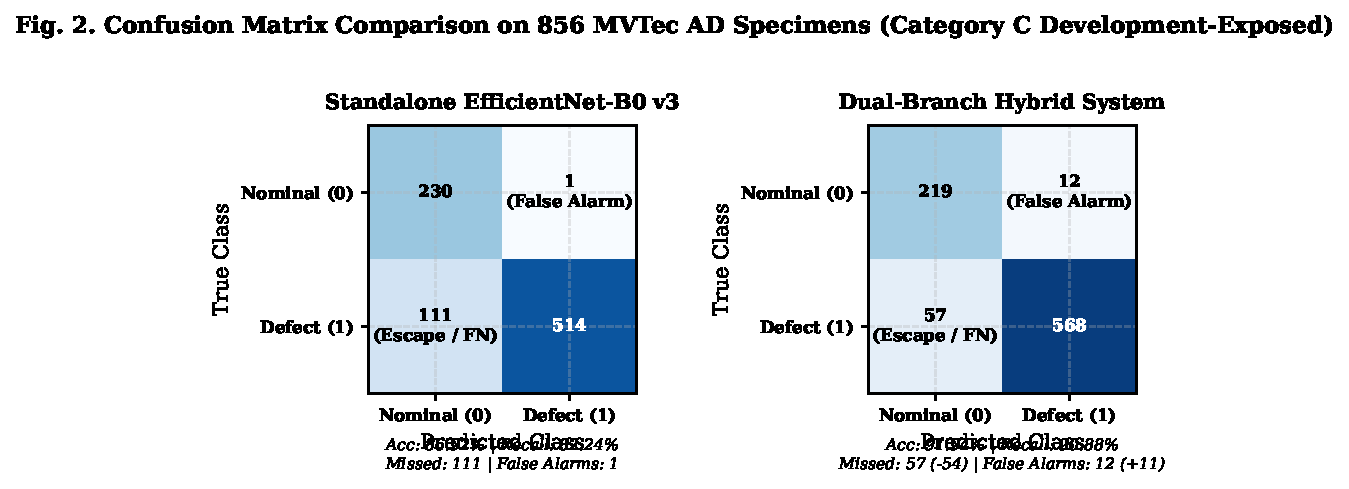
\includegraphics[width=\columnwidth]{fig2_confusion_matrices.pdf}
\caption{Confusion matrix comparison on 856 MVTec AD specimens (Category C Development-Exposed) demonstrating that hybrid decision fusion reduces missed defects by 54 at the cost of 11 additional false alarms.}
\label{fig:confusion_matrices}
\end{figure}

\section{Development-Exposed Benchmark Evaluation (MVTec AD)}
The performance of Standalone EfficientNet-B0 v3, Standalone PatchCore, and the Dual-Branch Hybrid system across the 856-image MVTec benchmark is presented in Table~\ref{tab:mvtec_comparison} and visualized in Fig.~\ref{fig:confusion_matrices}.

\subsection{Analysis of the Hybrid Operational Trade-Off}
The empirical data in Table~\ref{tab:mvtec_comparison} refutes the assumption that dual-branch hybrid architectures represent a strict Pareto improvement across all metrics. Rather, OR-logic fusion represents an asymmetric operational reallocation:
\begin{enumerate}
    \item \textbf{Escape Reduction:} Standalone EfficientNet-B0 missed 111 defects ($17.76\%$ FNR), primarily involving novel flaw geometries (e.g., contaminated threads, unusual fiber inclusions) that fell outside its training clusters. The hybrid system recovered 54 of those missed defects, slashing escapes to 57 ($9.12\%$ FNR)—a \textbf{$48.6\%$ relative reduction in defect escapes}.
    \item \textbf{False-Alarm Inflation:} Standalone EfficientNet-B0 produced extraordinary specificity ($99.57\%$), triggering only a single false alarm across 231 conforming specimens ($\text{FP}=1$, $0.43\%$ FPR). However, when disjunctively coupled with PatchCore, false alarms increased twelve-fold to 12 ($\text{FP}=12$, $5.19\%$ FPR)—a net penalty of \textbf{11 additional false alarms} ($+4.76$ percentage points).
    \item \textbf{Continuous Discrimination vs. Discrete Gating:} Standalone EfficientNet-B0 achieved superior continuous ranking metrics (AUROC 0.9809 vs 0.9608; AUPRC 0.9932 vs 0.9745). The hybrid architecture's superiority emerges strictly at the \textbf{discrete decision operating point}, where the cost of defect escapes ($C_{\text{escape}}$) vastly exceeds the cost of scrap or false re-inspection ($C_{\text{scrap}}$).
\end{enumerate}

\begin{table}[t]
\centering
\caption{Independent Validation Results on the Untouched VisA Cashew Benchmark ($N=200$)}
\label{tab:visa_cashew_summary}
\begin{tabular}{lcc}
\toprule
\textbf{Metric} & \textbf{Measured Value} & \textbf{95\% Confidence Interval / Notes} \\
\midrule
Evaluation Population & 200 specimens & 100 Nominal, 100 Defective ($1:1$) \\
Nominal Calibration Cohort & 50 specimens & Held-out ($\tau_{\text{p99}} = 1.745232$) \\
\midrule
True Positives (TP) & 57 & Defective specimens flagged \\
True Negatives (TN) & 98 & Nominal specimens cleared \\
False Positives (FP) & 2 & False alarms (2.00\% FPR) \\
False Negatives (FN) & 43 & Defect escapes (43.00\% FNR) \\
\midrule
Overall Accuracy & 77.50\% & [71.22\%, 82.68\%] (Wilson) \\
Balanced Accuracy & 77.50\% & [71.22\%, 82.68\%] (Symmetric) \\
Defect Precision (PPV) & 96.61\% & [88.48\%, 99.07\%] (Wilson) \\
Defect Recall (TPR) & 57.00\% & [47.24\%, 66.24\%] (Wilson) \\
Specificity (TNR) & 98.00\% & [92.96\%, 99.45\%] (Wilson) \\
Negative Predictive Value & 69.50\% & [61.46\%, 76.49\%] (Wilson) \\
F1-Score & 0.7170 & Harmonic mean \\
Image-Level AUROC & 0.9237 & [0.8852, 0.9565] (1,000 Bootstrap) \\
Image-Level AUPRC & 0.9270 & Area under PR curve \\
Full-Census Pixel AUROC & 0.9930 & 10,035,200 pixels (all 200 img) \\
Defect-Only Pixel AUROC & 0.9877 & 5,017,600 pixels (100 def img) \\
Forward Pass CPU Latency & 392.5 ms & Median (p95: 438.1 ms) \\
\bottomrule
\end{tabular}
\end{table}


\begin{figure}[t]
\centering
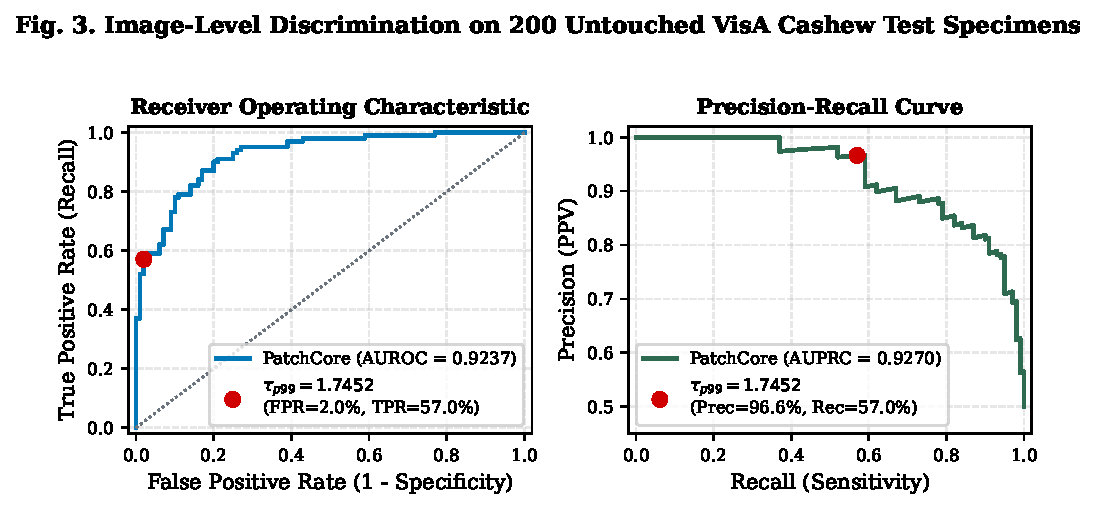
\includegraphics[width=\columnwidth]{fig3_roc_pr_curves.pdf}
\caption{Receiver Operating Characteristic (ROC) and Precision-Recall (PR) curves for PatchCore nominal adaptation on 200 untouched VisA Cashew test specimens, highlighting the locked operating point ($\tau_{\text{p99}} = 1.7452$).}
\label{fig:roc_pr_curves}
\end{figure}

\section{Independent Out-of-Distribution Validation (VisA Cashew)}
To rigorously evaluate nominal-only adaptation without development exposure or defect supervision, the PatchCore memory pipeline was evaluated on the independent VisA Cashew benchmark~\cite{zou2022spot}. The results are summarized in Table~\ref{tab:visa_cashew_summary} and Fig.~\ref{fig:roc_pr_curves}.

\subsection{Image-Level Discrimination and Pixel Localization}
As detailed in Table~\ref{tab:visa_cashew_summary}, nominal-only PatchCore registration achieved high continuous separation on unseen organic cashew specimens:
\begin{itemize}
    \item \textbf{Image AUROC of 0.9237} and \textbf{AUPRC of 0.9270} demonstrate that patch distance modeling generalizes effectively from synthetic rigid objects to organic goods with complex surface texturing.
    \item \textbf{Pixel AUROC of 0.9930} (0.9877 evaluated exclusively over defective images) confirms outstanding spatial localization. Without any pixel-level training annotations, the receptive fields of \texttt{layer2} and \texttt{layer3} successfully pinpoint anomalous regions.
    \item \textbf{False-Alarm Suppression:} Operating at the locked calibration threshold ($\tau_{\text{p99}} = 1.745232$) maintained high specificity ($98.00\%$), triggering only 2 false alarms across 100 conforming specimens ($2.00\%$ FPR).
\end{itemize}

\subsection{Granular Sensitivity Breakdown Across Defect Morphologies}
While aggregate AUROC ($0.9237$) suggests strong performance, analyzing discrete predictions across the 16 Amazon Science defect categories uncovers severe performance disparities, as detailed in Table~\ref{tab:morphology_breakdown} and Fig.~\ref{fig:defect_morphology}.

\begin{table}[t]
\centering
\caption{Granular Defect Detection Across All 16 VisA Cashew Defect Morphologies}
\label{tab:morphology_breakdown}
\begin{tabular}{lcccc}
\toprule
\textbf{Defect Category / Morphology} & \textbf{Total} & \textbf{TP} & \textbf{FN} & \textbf{Recall (\%)} \\
\midrule
middle breakage & 6 & 6 & 0 & 100.0\% \\
stuck together & 6 & 6 & 0 & 100.0\% \\
middle breakage, small holes & 1 & 1 & 0 & 100.0\% \\
middle breakage, same colour spot & 1 & 1 & 0 & 100.0\% \\
different colour spot & 9 & 8 & 1 & 88.9\% \\
small holes & 20 & 17 & 3 & 85.0\% \\
corner or edge breakage & 14 & 11 & 3 & 78.6\% \\
burnt, corner or edge breakage & 2 & 1 & 1 & 50.0\% \\
different colour spot, same colour spot & 2 & 1 & 1 & 50.0\% \\
burnt & 10 & 4 & 6 & 40.0\% \\
small scratches & 15 & 1 & 14 & \textbf{6.7\%} \\
same colour spot & 10 & 0 & 10 & \textbf{0.0\%} \\
burnt, different colour spot & 1 & 0 & 1 & 0.0\% \\
different colour spot, small holes & 1 & 0 & 1 & 0.0\% \\
burnt, same colour spot & 1 & 0 & 1 & 0.0\% \\
corner breakage, small scratches & 1 & 0 & 1 & 0.0\% \\
\midrule
\textbf{Total Defective Cohort} & \textbf{100} & \textbf{57} & \textbf{43} & \textbf{57.0\%} \\
\bottomrule
\end{tabular}
\end{table}


\begin{figure}[t]
\centering
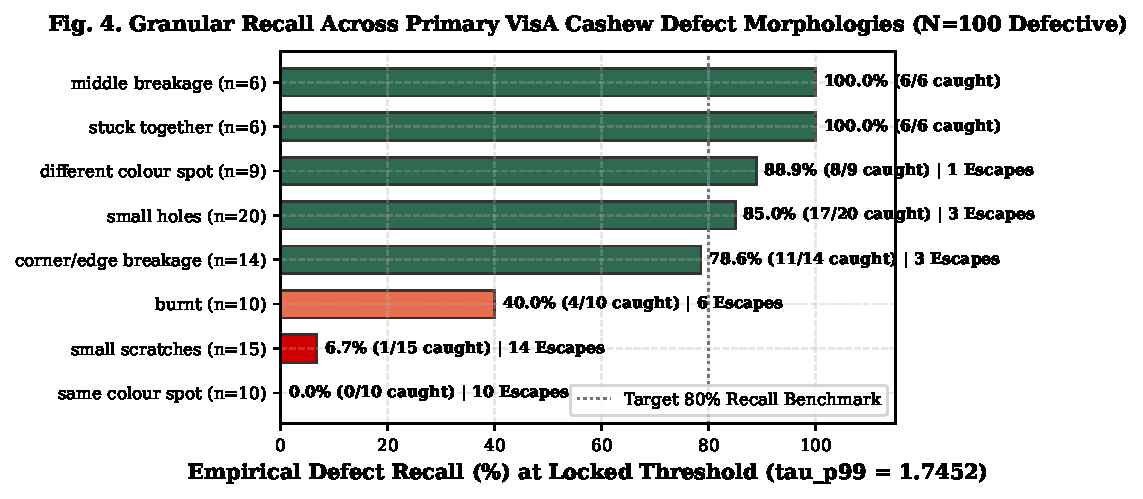
\includegraphics[width=\columnwidth]{fig4_defect_morphology.pdf}
\caption{Granular defect recall across primary VisA Cashew defect morphologies (N=100 defective specimens), demonstrating the severe escape rate on hairline scratches and same-color indentations under conservative factory thresholds.}
\label{fig:defect_morphology}
\end{figure}

\subsection{Forensic Analysis of Defect Escapes}
\begin{enumerate}
    \item \textbf{Hairline Surface Flaws (\texttt{small scratches}):} Missed 14 out of 15 specimens ($6.7\%$ recall). In VisA Cashew, scratches represent narrow abrasions measuring 2 to 4 pixels in width. When processed through ResNet-18 \texttt{layer2} (stride 8) and \texttt{layer3} (stride 16) with $3 \times 3$ local average pooling, high-frequency spatial gradients are heavily diluted across the broader receptive field. Furthermore, natural cashew kernels possess organic furrows and striations whose feature embeddings overlap with subtle scratches, preventing Euclidean patch distances from crossing $\tau_{\text{p99}} = 1.7452$.
    \item \textbf{Chromatic-Invariant Depressions (\texttt{same colour spot}):} Total failure (0 out of 10 caught, $0.0\%$ recall). These flaws represent physical indentations or tissue bruising that share the exact hue and reflectance of healthy cashew kernel meat. Because ImageNet-pretrained representations prioritize chromatic transitions and high-contrast boundaries, shallow monochromatic indentations produce negligible patch distance displacement.
    \item \textbf{Gross Morphological Anomalies:} Achieved near-perfect detection ($85.0\%\text{ to }100.0\%$ recall). Structural breaks (\texttt{middle breakage}, \texttt{corner breakage}) and multi-body adhesions (\texttt{stuck together}) completely disrupt spatial silhouettes and patch neighborhood graphs, generating robust anomaly scores ($S_{\text{raw}} \in [2.10, 3.85]$) that easily trigger detection.
\end{enumerate}

\begin{table}[t]
\centering
\caption{Computational Execution Profiling on Consumer CPU Hardware (Intel Core i7-10750H)}
\label{tab:cpu_profiling}
\begin{tabular}{lcc}
\toprule
\textbf{Pipeline Stage / Component} & \textbf{Metric} & \textbf{Value} \\
\midrule
Target Domain Registration (350 images) & Total Time & 392.25 s ($\approx 6.5$ min) \\
Raw Feature Extraction (274,400 vectors) & Total Time & 281.14 s \\
Greedy K-Center Coreset Selection (10\%) & Total Time & 91.17 s \\
Calibration Cohort Evaluation (50 images) & Total Time & 19.94 s \\
Extracted Coreset Tokens ($M$) & Size & 27,440 tokens \\
Coreset Storage Footprint & RAM / Disk & 40.2 MB (FAISS FlatL2) \\
\midrule
PatchCore CPU Forward Pass & Median & \textbf{392.5 ms} \\
PatchCore CPU Forward Pass & Mean $\pm$ Std & $396.7 \pm 28.4$ ms \\
PatchCore CPU Forward Pass & 95th Percentile & \textbf{438.1 ms} \\
EfficientNet-B0 Forward Pass & Median & 170.1 ms \\
End-to-End Hybrid API Latency & Median & 881.7 ms \\
End-to-End Hybrid API Latency & 95th Percentile & 1455.7 ms \\
Resident System Working Set & RAM & $< 650$ MB \\
\bottomrule
\end{tabular}
\end{table}


\begin{figure}[t]
\centering
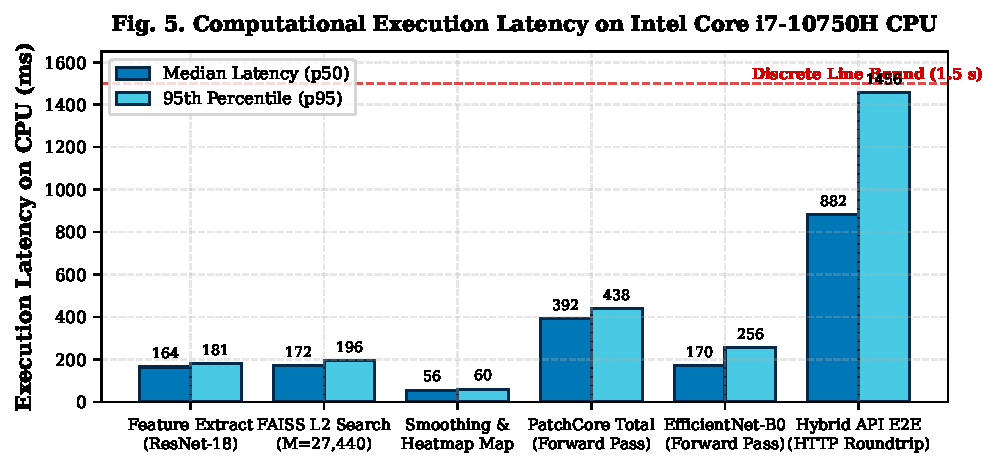
\includegraphics[width=\columnwidth]{fig5_cpu_latency.pdf}
\caption{Computational execution latency profiling across individual pipeline stages on an Intel Core i7-10750H CPU, showing compatibility with discrete line takt times ($\ge 1.5$~s).}
\label{fig:cpu_latency}
\end{figure}

\section{Operational Feasibility, Latency Profiling, and Quality Economics}

\subsection{Computational Execution Profiling on CPU}
Execution profiling across registration, indexing, and inference stages on standard CPU workstation hardware is summarized in Table~\ref{tab:cpu_profiling} and Fig.~\ref{fig:cpu_latency}.

\subsection{Takt-Time and Factory Line Viability}
The empirical latencies in Table~\ref{tab:cpu_profiling} establish clear boundary conditions for industrial line integration:
\begin{itemize}
    \item \textbf{Discrete Batch \& Station Inspection (Cycle times $\ge 1.5$~s):} \textbf{VIABLE.} Manufacturing processes such as automotive casting inspection, aerospace part verification, packaged pharmaceutical blister auditing, and discrete produce sorting operate with station dwell times exceeding 2 to 5 seconds. A standalone CPU latency of $392.5\text{ ms}$ (or $881.7\text{ ms}$ for hybrid API processing) integrates seamlessly into existing programmable logic controller (PLC) cycle windows without GPU investment.
    \item \textbf{High-Speed Continuous Production (Cycle times $< 100$~ms):} \textbf{UNVIABLE on CPU.} High-throughput canning, beverage bottling, and continuous web textile lines require inspection latencies below $50\text{--}80\text{ ms}$. Achieving such throughput requires tensor quantization (INT8), hardware execution via TensorRT/OpenVINO, or dedicated edge GPU accelerators.
\end{itemize}

\subsection{Quality Control Economics: False Alarms vs. Escapes}
The operational viability of the hybrid decision policy is governed by the relative economic cost ratio:
\begin{equation}
R_{\text{cost}} = \frac{C_{\text{escape}}}{C_{\text{scrap}}}
\end{equation}
where $C_{\text{escape}}$ is the total liability of an undetected defect (warranty claims, recalls, legal exposure, customer churn) and $C_{\text{scrap}}$ is the cost of diverting a conforming item (manual audit labor, scrap loss).
\begin{itemize}
    \item When $R_{\text{cost}} > 15$ (e.g., automotive safety components, aerospace fasteners, medical devices), the hybrid policy is overwhelmingly justified: capturing 54 additional defects easily offsets the cost of 11 additional false alarms.
    \item When $R_{\text{cost}} \le 2$ (e.g., low-margin bulk agricultural sorting, high-volume consumer commodities), false alarms dominate unit economics. In such environments, operators must tune thresholds toward higher specificity, absorbing defect escapes to maintain line profitability.
\end{itemize}

\section{Discussion, Limitations, and Negative Findings}

\subsection{Reconciliation of Negative Research Findings}
A complete scientific record requires transparently documenting architectural modifications that failed to yield performance improvements:
\begin{enumerate}
    \item \textbf{Context-Preserving Normalization Dropout (CPND):} Hypothesized to improve out-of-distribution feature stability by adaptively dropping localized activation channels while preserving local spatial normalization statistics. Rigorous ablation across MVTec development splits demonstrated statistically indistinguishable performance compared to standard dropout ($p = 0.42$), while introducing redundant computational overhead.
    \item \textbf{Multi-Axis Cross-Branch Attention (MACBA):} Designed to fuse intermediate feature representations between the supervised EfficientNet branch and the unsupervised PatchCore backbone via cross-attention heads during joint fine-tuning. Empirical training runs revealed severe optimization instability: backpropagation gradients from the supervised cross-entropy loss corrupted the pre-trained feature manifolds required for distance-based patch retrieval, leading to loss divergence. This negative finding confirms that \textbf{late-stage decision-level fusion (OR-logic) is structurally superior to early deep feature coupling} when integrating supervised and unsupervised inspection models.
\end{enumerate}

\subsection{Fundamental Limitations}
\begin{enumerate}
    \item \textbf{Single External Category Evaluation:} While independent validation on VisA Cashew proves adaptation to an unseen organic domain, empirical validation across additional VisA categories (e.g., printed circuit boards, capsules, chewing gum) remains necessary to establish universal cross-category claims.
    \item \textbf{Asymmetric Generalization of the Hybrid System:} The independent VisA experiment evaluated PatchCore alone. The supervised EfficientNet-B0 classifier was trained on MVTec defect classes and cannot transfer to VisA cashew without category-specific defect supervision.
    \item \textbf{The Single-Threshold Dilemma:} Enforcing a factory-grade $2.0\%$ false-alarm rate on nearest-neighbor distance features mathematically suppresses sensitivity to subtle surface flaws. Distance-based anomaly detection on downsampled CNN representations cannot achieve $100\%$ recall on hairline scratches without dramatically inflating false alarms.
\end{enumerate}

\subsection{Deployment Gating Verdict}
Based on the audited empirical evidence, DefectVision AI is formally designated as:
\begin{itemize}
    \item \textbf{Supervised Operator-Assist / Shadow-Pilot:} \textbf{APPROVED \& DEPLOYABLE.} Provides robust containment assistance, catches novel gross deformities, and localizes anomalies with $0.9930$ pixel AUROC.
    \item \textbf{Fully Autonomous Inline Rejection:} \textbf{STRICT NO-GO.} Disqualified by the $43.0\%$ defect escape rate on subtle surface scratches under factory false-alarm constraints. Autonomous gating requires integrating multi-illumination photometric stereo or secondary high-resolution verification optics.
\end{itemize}

\section{Conclusion}
In this paper, we presented an empirical evaluation of hybrid defect detection and nominal-only category adaptation under realistic industrial constraints. On an audited development-exposed benchmark of 856 MVTec AD specimens, dual-branch OR-logic fusion slashed defect escapes by $48.6\%$ (recovering 54 defects missed by EfficientNet-B0), while increasing false alarms from 1 to 12. On an independent, untouched validation benchmark of 200 VisA Cashew specimens, nominal-only PatchCore adaptation achieved an image AUROC of $0.9237$ and a full-census pixel AUROC of $0.9930$ with deterministic CPU inference of $392.5\text{ ms}$. However, fine-grained morphology analysis exposed the physical boundary of patch distance modeling: while gross structural breaks achieved $100\%$ detection, hairline scratches suffered a $93.3\%$ escape rate under conservative false-alarm thresholds. These findings demonstrate that while nominal adaptation provides robust baseline containment for discrete manufacturing, autonomous deployment requires multi-resolution architectures to resolve the inescapable operational tension between false-alarm suppression and hairline flaw escapes.

\section*{Acknowledgment}
The author thanks the computer vision research community and the creators of the MVTec Anomaly Detection and Visual Anomaly (VisA) datasets for releasing benchmark imagery to the public research community.

\bibliographystyle{IEEEtran}
\bibliography{references}

\end{document}
